


\subsection{Datasets description}

\textbf{\mnist-\svhn}  \cite{mmvaeShi2019} is constructed using pairs of \mnist and \svhn, sharing the same digit class (See \Cref{fig:ms_dataset}). Each instance of a digit class (in either dataset) is randomly paired with 20 instances of the same digit class from the other data-set. \svhn modality samples are obtained from house numbers in Google Street View images, characterized by a variety of colors, shapes and  angles. A high number of \svhn samples are noisy and can contain different digits within the same sample due to the imperfect cropping of the original full house number image. One challenge of this data-set for multi-modal generative models is to learn to extract digit number and reconstruct a coherent \mnist modality.

\textbf{\mhd}  \cite{Vasco2022} is composed of 3 modalities: synthetically generated images and motion trajectories of handwritten digits associated with their speech sounds. The images are gray scale $1 \cross 28 \cross 28$ and the handwriting trajectory are represented by a $1 \cross 200$ vector. The spoken digits sound is $1s$ long audio processed as Mel-Spectrograms constructed with a hopping window of $512$ ms with $128$ Mel Bins  resulting in a $1 \cross 128 \cross 32$ representation. This benchmark is the closest to a real world multi-modal sensors scenario because of the presence of three completely different modalities, the audio modality representing a complex data type. Therefore, similar to \svhn, the conditional generation of sound to coherent images or trajectories represents a challenging use case.

\textbf{\polymnist} \cite{sutter2021generalized} is an extended version of the \mnist data-set to 5 modalities. Each modality is constructed using a randomly set of \mnist digits with an overlay over a random crop from a modality specific, 3 channel image background. This synthetic generated data-set allows the evaluation of the scalability of multi-modal generative models to large number of modalities. Although this data-set is composed of only images, the different modality-specific background having different textures, results in different levels of difficulty. In \Cref{fig:datasets_mmnist}, the digits numbers are more difficult to distinguish in modality 1 and 5 than in the remaining modalities.


\textbf{\cub} \cite{mmvaeShi2019} is comprised of bird images and their associated text captions. The work in \cite{mmvaeShi2019} used a simplified version based on pre-computed ResNet-features. We follow \cite{Daunhawer2021} and conduct all our experiments on the real image data instead. Each image from the 11,788 photos of birds from Caltech-Birds \cite{wah2011caltech} are resized to $ 3 \cross 64 \cross 64 $ image size and coupled with 10 textual descriptions of the respective bird (See \Cref{fig:cub_d}).


\begin{figure}[h]
     \centering
     \begin{subfigure}[b]{0.3\linewidth}
      \centering
         \begin{subfigure}{1.0\linewidth}
             \centering
             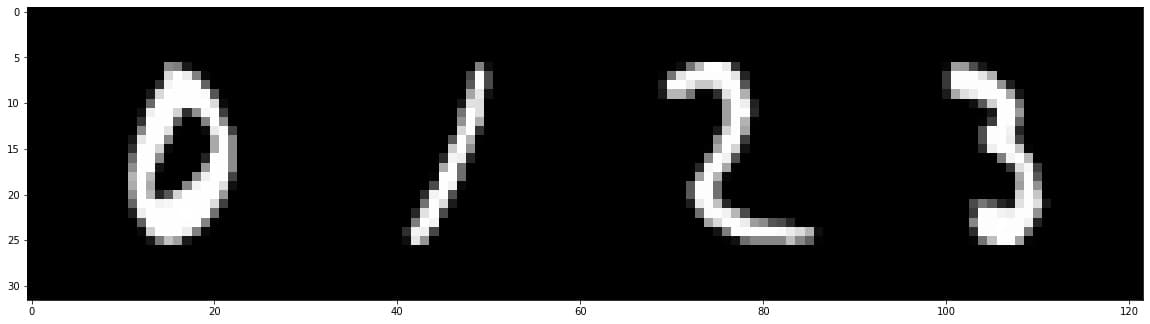
\includegraphics[width=1.4in]{figures/datasets/ms/dataset_mnist}
             \caption*{\mnist}
         \end{subfigure}
         \begin{subfigure}{1.0\linewidth}
             \centering
             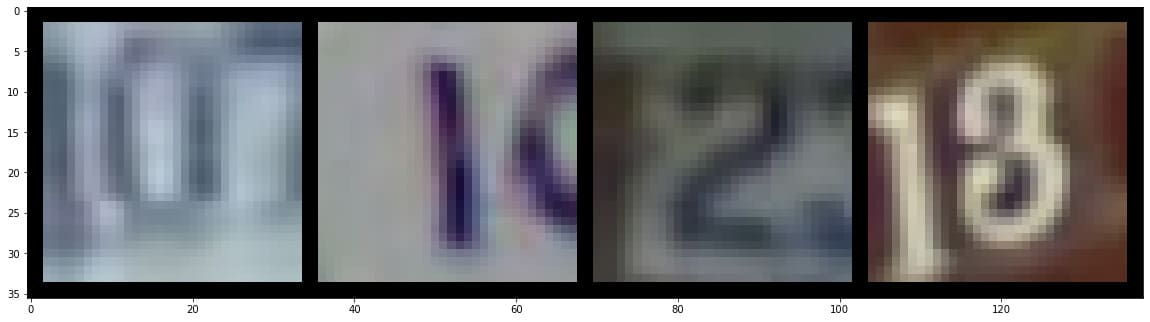
\includegraphics[width=1.4in]{figures/datasets/ms/dataset_svhn}
             \caption*{\svhn}
         \end{subfigure}
        \caption{\textbf{\mnist-\svhn} }\label{fig:ms_dataset}
    \end{subfigure}
     \begin{subfigure}[b]{0.3\linewidth}
      \centering
         \begin{subfigure}{1.0\linewidth}
             \centering
             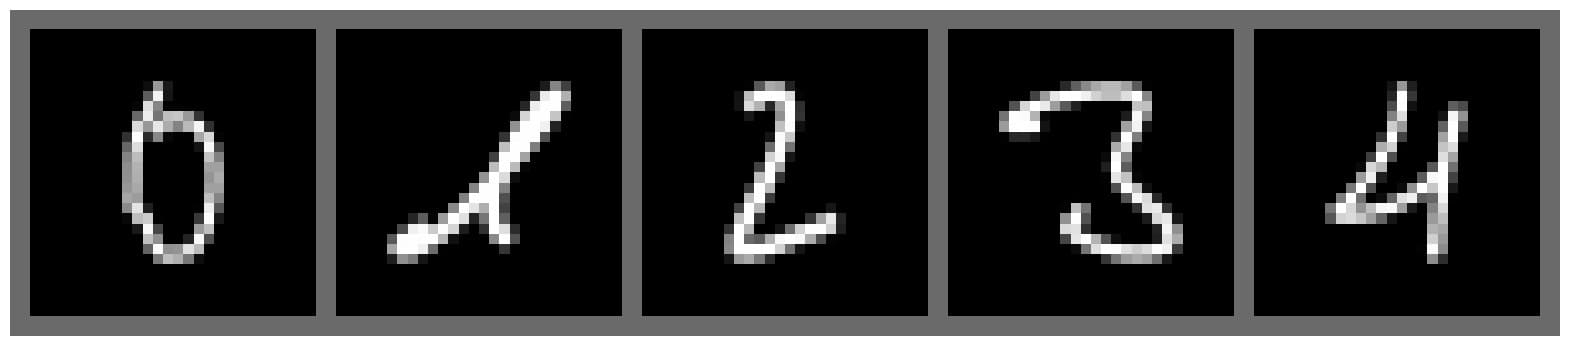
\includegraphics[width=1.4in]{figures/datasets/mhd/image_dataset}
             \label{fig:mjd_image}
             \caption*{Image}
         \end{subfigure}
         \begin{subfigure}{1.0\linewidth}
             \centering
             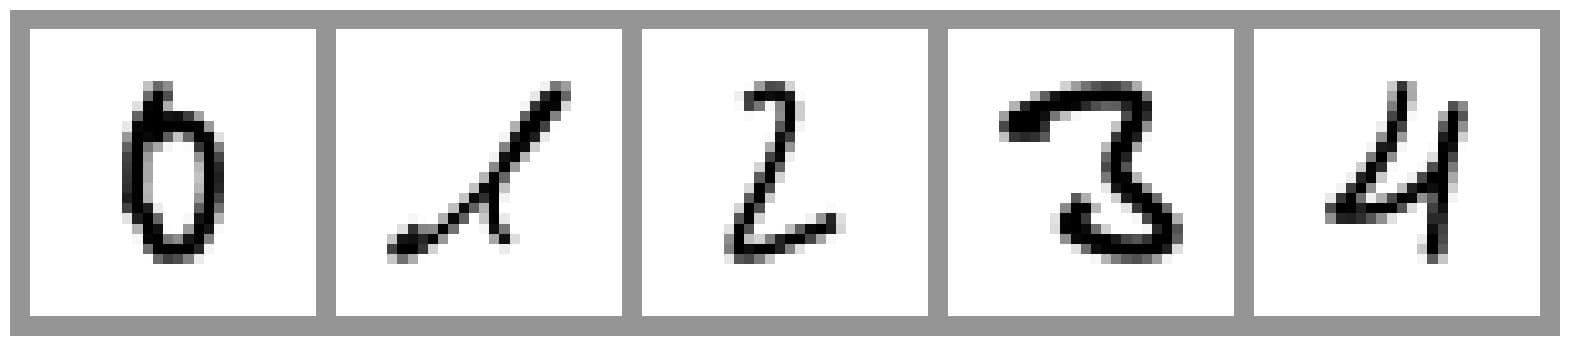
\includegraphics[width=1.4in]{figures/datasets/mhd/traj_dataset}
             \label{fig:mhd_traj}
             \caption*{Trajectory}
         \end{subfigure}
        \begin{subfigure}{1.0\linewidth}
             \centering
             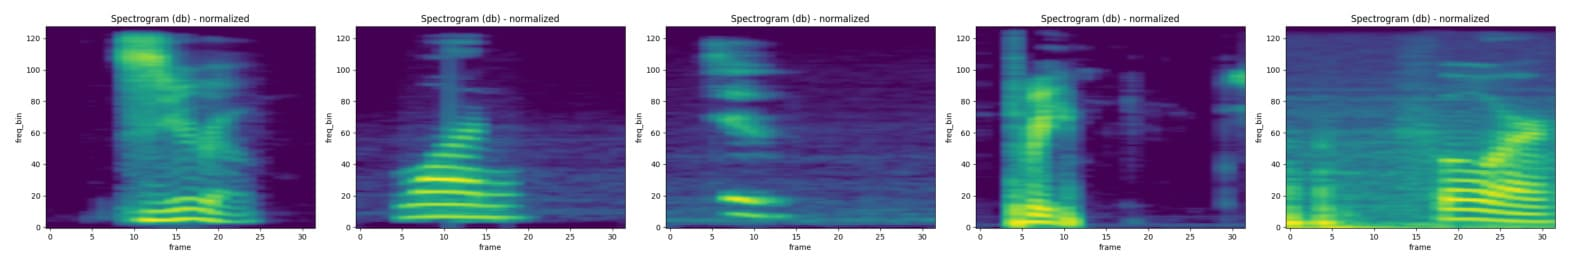
\includegraphics[width=1.4in]{figures/datasets/mhd/sound_dataset}
             \label{fig:mhd_sound}
             \caption*{Sound Mel-Spectogram}
         \end{subfigure}
        \caption{\textbf{\mhd}}
    \end{subfigure}
    \begin{subfigure}[b]{0.3\linewidth}
     \centering
         \begin{subfigure}{1.0\linewidth}
             \centering
             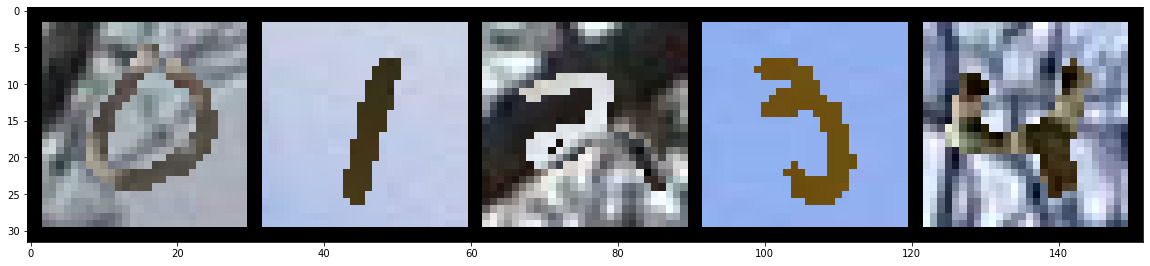
\includegraphics[width=1.4in]{figures/datasets/mmnist/dataset_m0}
             \label{fig:mm0}
             
         \end{subfigure}
          \begin{subfigure}{1.0\linewidth}
             \centering
             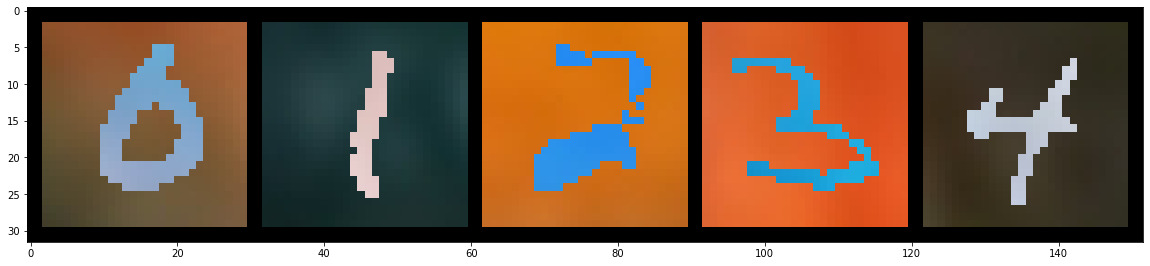
\includegraphics[width=1.4in]{figures/datasets/mmnist/dataset_m1}
             \label{fig:mm1} 
          
         \end{subfigure}
          \begin{subfigure}{1.0\linewidth}
             \centering
             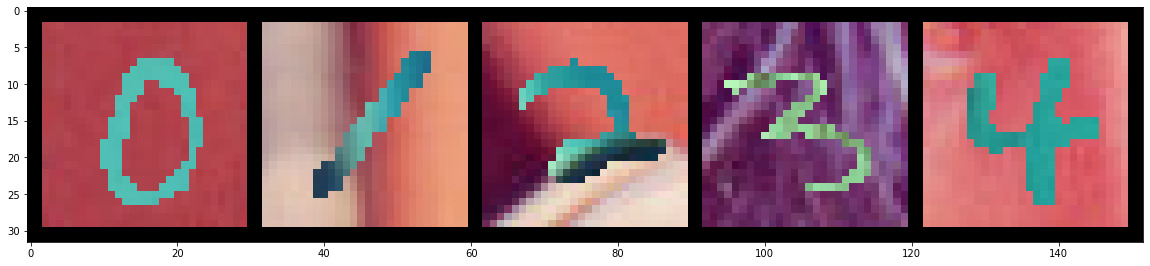
\includegraphics[width=1.4in]{figures/datasets/mmnist/dataset_m2}
             \label{fig:mm2}
             
         \end{subfigure}
           \begin{subfigure}{1.0\linewidth}
             \centering
             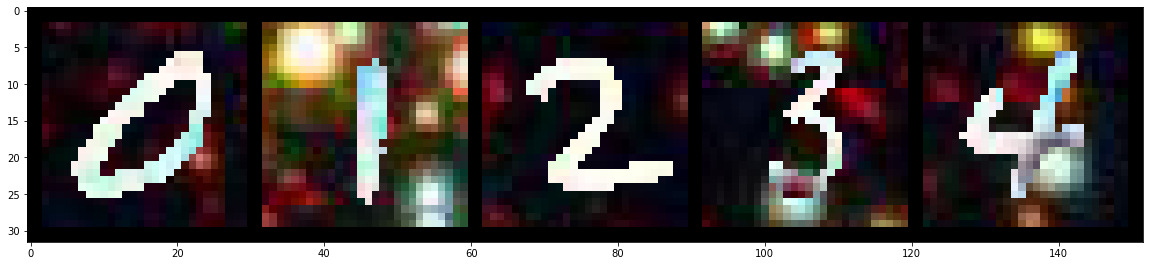
\includegraphics[width=1.4in]{figures/datasets/mmnist/dataset_m3}
             \label{fig:mm3}
         \end{subfigure}
           \begin{subfigure}{1.0\linewidth}
             \centering
             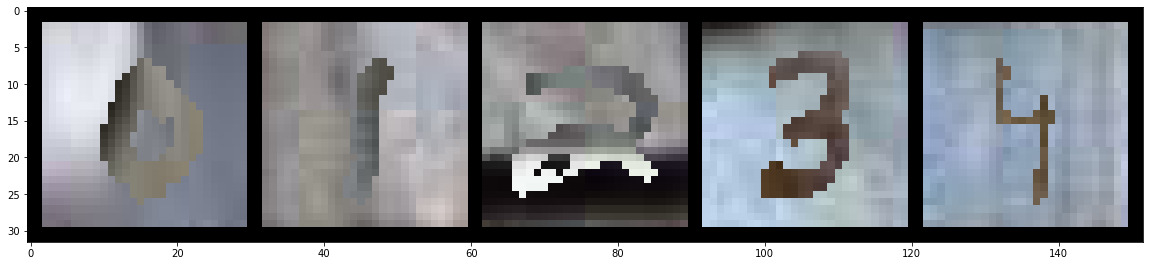
\includegraphics[width=1.4in]{figures/datasets/mmnist/dataset_m4}
             \label{fig:mm4}
             
         \end{subfigure}
            \caption{\textbf{ \polymnist}} \label{fig:datasets_mmnist}
            
    \end{subfigure}
    
       \begin{subfigure}{0.5\linewidth}
             \centering
             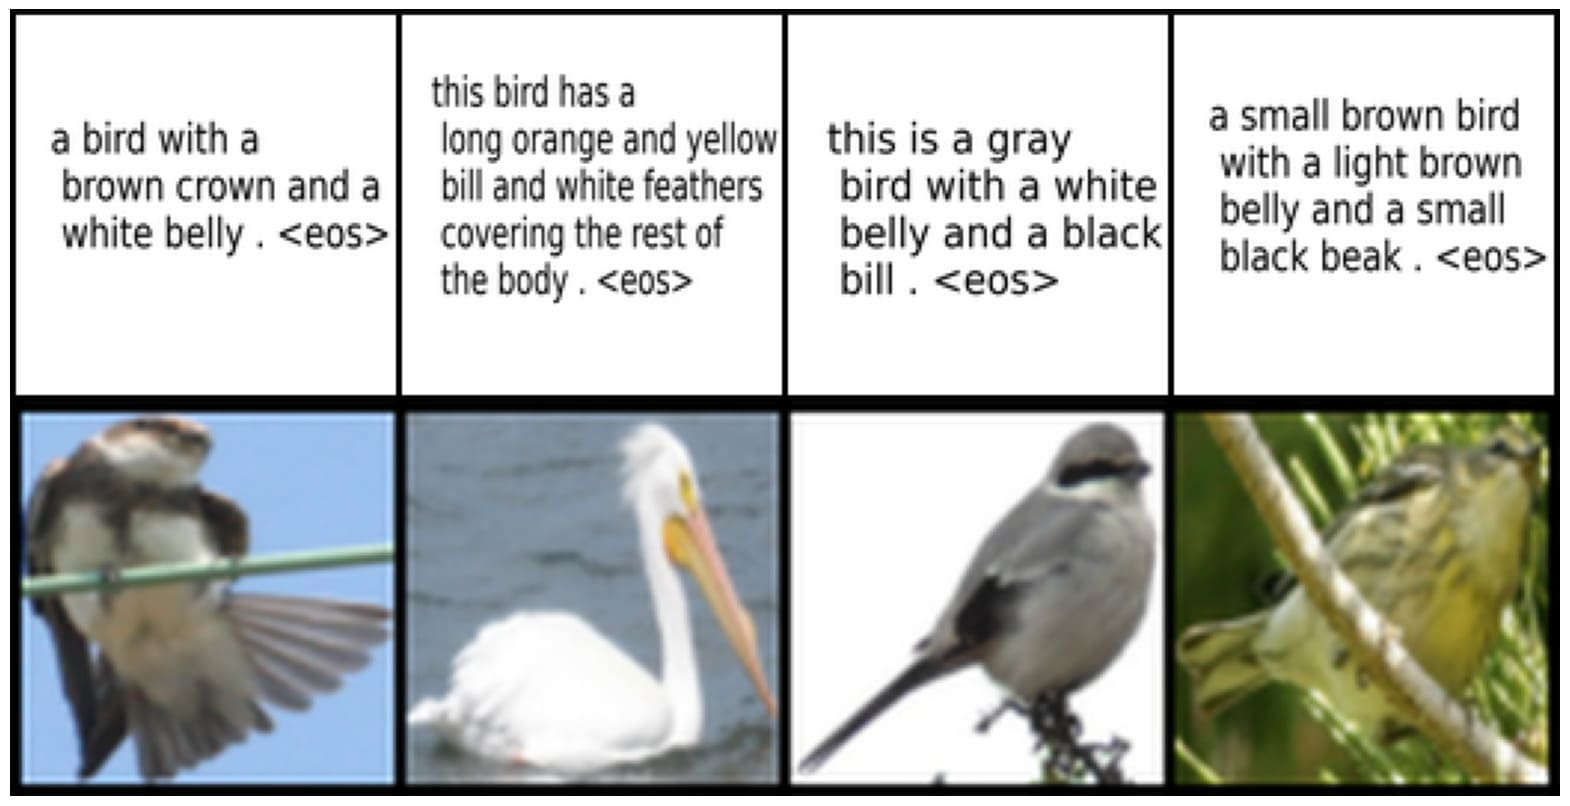
\includegraphics[width=1.4in]{figures/datasets/cub/dataset}
             \caption{\textbf{ \cub}}
             \label{fig:cub_d}
             
         \end{subfigure}
        \caption{Illustrative example of the Datasets used for the evaluation }\label{fig:datasets}
\end{figure}

\subsection{Evaluation metrics}
Multimodal generative models are evaluated in terms of generative coherence and quality.

 



\subsubsection{Generation Coherence}
\label{apdx:eval_coh}
%% formalize the coherence accuracy in general
 We measure \textit{coherence} by verifying that generated data (both for joint and conditional generations) share the same information across modalities. Following \cite{mmvaeShi2019, sutter2021generalized, tcmvaehwang21,Vasco2022,Daunhawer2021}, we consider the class label of the modalities as the shared information and use pre-trained classifiers to extract the label information form the generated samples and compare it across modalities. 


For \textbf{\mnist-\svhn} , \textbf{\mhd}  and \textbf{\polymnist}, the shared semantic information is the digit class number. Single modality classifiers are trained to classify the digit number of a given modality sample. To compute the conditional generation of modality $m$ with a subset of modalities $A$, we feed the modality specific pre-trained classifier $\mathbf{C}_m$ with the conditional generated sample $\hat{X}^m$. The predicted label class is compared to the ground truth label $y_{X^{A}}$ which is the label of modalities of the subset $X^{A}$. For $N$ samples, the matching rate average establishes the coherence. For all the experiments, $N$ is equal to the length of the test-set.
\begin{equation}
    \textit{Coherence}( \hat{X}^m | X^{A}  ) = \frac{1}{N} \sum_1^N \mathds{1}_{ \{ \mathbf{C}_m ( \hat{X}^m) = y_{X^{A}} \}}  
\end{equation}

The \textbf{joint generation coherence} is measured by feeding the generated samples of each modality to their specific trained classifier. The rate with which all classifiers output the same predicted digit label for $N$ generations is considered as the joint generation coherence. 

\textbf{The leave one out coherence:} is the conditional generation coherence using all the possible subsets excluding the generated modality: $\textit{Coherence}( \hat{X}^m | X^A  )$ with $A= \{1,..,M \} \setminus m $ ).
Due to the large number of modalities in \textbf{\polymnist}, similar to  \cite{ sutter2021generalized, tcmvaehwang21,Daunhawer2021}  we compute the average \textbf{leave one out coherence} conditional coherence as a function of the input modalities subset size.


Due to the unavailability of labels in the \textbf{\cub} data-set, we use \gls{CLIP-S} \cite{hessel2021clipscore} a state of the art metric for image captioning evaluation.

%% talk about clip score


\subsubsection{Generation Quality}
For each modality, we consider the following metrics: 
\begin{itemize}
    \item \textbf{RGB Images}: \gls{FID} \cite{fid} is the  state-of-the-art standard metric to evaluate image generation quality of generative models.
    \item \textbf{Audio}: \gls{FAD} \cite{fad},  is state-of-the-art standard metric in the evaluation of audio generation. \gls{FAD} performs well in terms of robustness against noise and is consistent with human judgments \cite{audiomet}. Similar to \gls{FID}, a Fréchet distance is computed but VGGish (audio classifer model) embeddings are used instead.
    \item \textbf{Other modalities} For other modality types, we derive \gls{FMD} (Fréchet Modality Distance), a similar metric to  \gls{FID} and \gls{FAD}. We compute the \textbf{Fréchet distance} between the statistics retrieved from the activations of the modality specific pre-trained classifiers used for coherence evaluation. \gls{FMD} is used to evaluate the generative quality of \mnist modality in \textbf{\mnist-\svhn} and image and trajectory modalities in \textbf{\mhd} data-set.
\end{itemize}
For conditional generation, we compute the quality metric (\gls{FID},\gls{FAD} or \gls{FMD}) using the conditionally generated modality and the real data. For joint generation, we use the randomly generated modality and randomly selected same number of samples from the real data.

 For \textbf{\cub}, we use $10000$ samples to evaluate the generation quality in terms of \gls{FID}.
In the remaining experiments, we use $5000$ samples to evaluate the performance in terms of \gls{FID}, \gls{FAD} or \gls{FMD}.




